\documentclass{beamer}
\usepackage{amsmath,amsfonts,amssymb,mathtools,ascmac,bm,fancybox,calc,multicol,physics,array}
\usepackage{graphicx,color}
\usepackage{tikz,listings,wrapfig,float,xcolor}
\usepackage{url,subcaption,multirow}
\usepackage{luatexja-fontspec}
    \usetikzlibrary{intersections,calc,arrows.meta,backgrounds,shapes.geometric,shapes.misc,positioning,fit,graphs,arrows}
    \setlength{\columnsep}{5mm}
\tikzset{file/.style={rectangle,rounded corners,draw,text centered,minimum height=1cm,text width=2.5cm}}
\tikzset{user/.style={draw,rounded corners,text centered}}
\usetheme{Madrid} 
%\usecolortheme[RGB={255,240,245}]{structure}
%\setbeamercolor{palette primary}{fg=black}
%\setbeamercolor*{palette secondary}{bg=white,fg=black}
%\setbeamercolor*{palette tertiary}{bg=white,fg=black}
%\setbeamercolor*{palette quaternary}{bg=white,fg=black}
\setbeamertemplate{navigation symbols}{}
\usefonttheme{professionalfonts}
    \renewcommand{\thefootnote}{\fnsymbol{footnote}}
\renewcommand{\figurename}{Fig\ }
\renewcommand{\tablename}{Tbl}
\newcommand{\figref}[1]{Fig\ \ref{#1}}
\newcommand{\tabref}[1]{Tbl\ \ref{#1}}
\makeatletter
\renewcommand{\thefigure}{%
\thesection.\arabic{figure}}
\@addtoreset{figure}{section}
\renewcommand{\thetable}{%
\thesection.\arabic{table}}
\@addtoreset{table}{section}
\@addtoreset{lstlisting}{section}
\@addtoreset{footnote}{page}
\makeatother


\title{Cryptography Basics}
\subtitle{Cryptography And Authentication}
\author[K.MIZOGUCHI]{MIZOGUCHI Koki\ \thanks{Infromation Security System Lab.}}
\date{\today}
\institute[KUT]{Kochi University of Technology}
\titlegraphic{\includegraphics[scale=0.3]{KUTLogo.jpg}}
\newcommand{\shownum}{\thesection\ -\ \thesubsection.\ }

\begin{document}
\begin{frame}
    \titlepage
\end{frame}
\section{Infomation security}
\begin{frame}{Table of Contents}
    \tableofcontents
\end{frame}
\subsection{Three elements of information security}
\newcommand{\threeelementsofinformationsecutiry}{\shownum Three elements of information security}
\begin{frame}
    % \frametitle{Table of Contents}
    \tableofcontents[currentsection,sectionstyle=show/shaded,subsectionstyle=shaded/shaded]
\end{frame}
\begin{frame}
    \frametitle{\threeelementsofinformationsecutiry}
    The following three are called the "three elements if information security"
    \begin{block}{}
        \begin{itemize}
            \item Confidentiality
            \item Integrity
            \item Availability
        \end{itemize}
    \end{block}
\end{frame}
\begin{frame}
    \frametitle{\threeelementsofinformationsecutiry}
    \begin{exampleblock}{Confidentiality}
        \textbf{Unauthorized persons should not have access to the information.}
    \end{exampleblock}
    \begin{exampleblock}{Integrity}
        \textbf{Information remains accurate and unaltered or erased.}
    \end{exampleblock}
    \begin{exampleblock}{Availability}
        \textbf{Authorized persons should be able to access information whenever they want.}
    \end{exampleblock}
\end{frame}
\begin{frame}
    \frametitle{\threeelementsofinformationsecutiry}
    \begin{table}
        \centering
        \renewcommand{\arraystretch}{1.5}
        \begin{tabular}{cll}
            \hline
            Requirement     & \multicolumn{1}{c}{Characteristics required} & \multicolumn{1}{c}{Cryptography}                  \\
            \hline
            Confidentiality & Data Privacy                                 & Encryption, Authentication                        \\
            Integrity       & Data Accuracy                                & {\footnotesize message authentication, signature} \\
            Availability    & Ease of access to data                       & secret sharing                                    \\
            \hline
        \end{tabular}
    \end{table}
\end{frame}
\subsection{Definition of Information Security}
\begin{frame}{\shownum Definition of Information Security}
    \begin{block}{}
        Information security is defined in {\it JIS Q 27000}\ \footnote{JIS(Japanese Industrial Standards) is national standard of Japan for standardization of Japanese industry.}.
    \end{block}
    \begin{block}{}
        {\it JIS Q 27000} states that {"Information security is the maintenance of confidentiality, integrity, and availability of information"}.
    \end{block}
\end{frame}
\subsection{Additional Requirements}
\newcommand{\additionalrequirements}{\shownum Additional Requirements}
\begin{frame}
    \frametitle{\additionalrequirements}
    When handling more sensitive information, the following requirements should be considered in addition to the three elements of information security.
    \begin{block}{}
        \begin{itemize}
            \item Authenticity
            \item Accoutability
            \item Non-repudiation
            \item Reliability
        \end{itemize}
    \end{block}
\end{frame}
\begin{frame}
    \frametitle{\additionalrequirements}
    \begin{exampleblock}{Authenticity}
        \textbf{The user or system is really the person and system, and no imposters are mixed in.}
    \end{exampleblock}
    \begin{exampleblock}{Accountability}
        \textbf{When a system behaves strangely or is attacked, it should be possible to trace what happened and why.}
    \end{exampleblock}
\end{frame}
\begin{frame}
    \frametitle{\additionalrequirements}
    \begin{exampleblock}{Non-repudiation}
        \textbf{Transactins, registrations, and other operations should not be later pretended to be something they are not.}
    \end{exampleblock}
    \begin{exampleblock}{Reliability}
        \textbf{The system is operating correctly and without any defects.}
    \end{exampleblock}
\end{frame}
\section{Encryption}
\begin{frame}
    \tableofcontents[currentsection,sectionstyle=show/shaded,subsectionstyle=shaded/shaded]
\end{frame}
\subsection{What is Cryptography?}
\begin{frame}{\shownum What is Cryptography?}
    \begin{exampleblock}{Encrypt}
        The information should be in a form that cannot seen by a third party.
    \end{exampleblock}
    \begin{exampleblock}{Decrypt}
        Converting chiphertext back to plaintext.
    \end{exampleblock}
    \begin{figure}
        \centering
        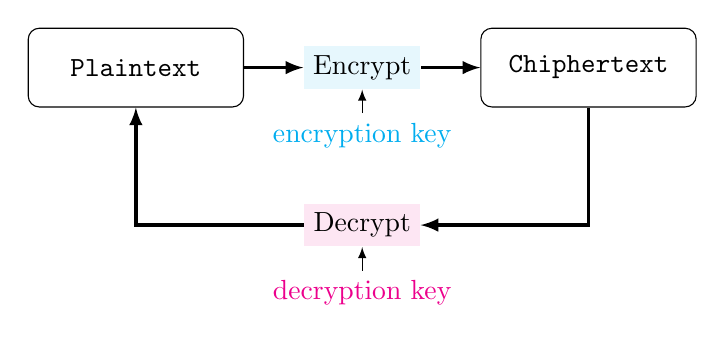
\begin{tikzpicture}
            \node[file](pt){\tt {Plaintext}};
            \node[file,right=3cm of pt](ct){\tt {Chiphertext}};
            \node[fill=cyan!10] at ($(pt)!0.5!(ct)$)(ec){Encrypt};
            \node[below=0.3cm of ec,cyan](ek){encryption key};
            \draw[-latex,very thick](pt)--(ec);
            \draw[-latex,very thick](ec)--(ct);
            \draw[-latex](ek)--(ec);
            \coordinate (pt2) at ($(pt)+(0,-2cm)$);
            \coordinate (ct2) at (ct |- pt2);
            \node[fill=magenta!10] at ($(pt2)!0.5!(ct2)$)(dc){Decrypt};
            \node[magenta,below=0.3cm of dc](dk){decryption key};
            \draw[-latex,very thick](dc)-|(pt);
            \draw[-latex,very thick](ct)|-(dc);
            \draw[-latex](dk)--(dc);
        \end{tikzpicture}
    \end{figure}
\end{frame}
\subsection{Decoding}
\begin{frame}{\shownum Decoding}
    \begin{exampleblock}{Decoding}
        Obtaining plaintext information in a way that was not intended by the chipher developer, without following a legitimate decryption process.
    \end{exampleblock}
\end{frame}
\section{Authentication}
\begin{frame}
    \tableofcontents[currentsection,sectionstyle=show/shaded,subsectionstyle=shaded/shaded]
\end{frame}
\subsection{Password Authentication}
\begin{frame}{\shownum Password Authentication}
    \begin{exampleblock}{Authentication}
        A process by which a person confirms to another person that he or she is indeed that person.
    \end{exampleblock}
    \begin{block}{Password or Passphrases}
        Passphrase is more strong.
        \begin{table}
            \centering
            \renewcommand{\arraystretch}{1.5}
            \begin{tabular}{llcl}
                % \hline
                \multicolumn{1}{c}{System} & \multicolumn{1}{c}{Pattern example} & Number of combinations & \multicolumn{1}{c}{example}    \\
                \hline
                Password                   & 8 characters                        & \(62^8\)               & {\tt P1kAIMiG}                 \\
                Passphrase                 & 4 words\ \footnotemark              & \(4000^4\)             & {\scriptsize \tt we map as ps}
            \end{tabular}
        \end{table}
        \footnotetext[1]{\ from 4000 words}
    \end{block}
\end{frame}
\subsection{Password Attack Techniques}
\newcommand{\framename}{\shownum Password Attack Techniques}
\begin{frame}{\framename}
    The following are the main password attack techniques.
    \begin{block}{}
        \begin{itemize}
            \setlength{\itemsep}{0.5cm}
            \item Dictionary attack
            \item Brute-force attack
            \item Reverse burute-force attack
            \item Password spray attack
            \item Password list attack
        \end{itemize}
    \end{block}
\end{frame}
\begin{frame}{\framename}
    \begin{exampleblock}{Dictionary attack}
        Obtain a list of popular passwords and try them one after the other.
    \end{exampleblock}
    \begin{exampleblock}{Blute-force attack}
        Fix the ID of a user and try passwords in order.
    \end{exampleblock}
    \begin{exampleblock}{Reverse blute-force attack}
        Fix the password and try ID in order.
    \end{exampleblock}
    \begin{exampleblock}{Password spray attack}
        Based on a large number of ID information, for each ID, try the same password in order.
    \end{exampleblock}
\end{frame}
\begin{frame}{\framename}
    \begin{exampleblock}{Password list attack}
        When one service is attacked and the password is leaked, the other service may also be attacked by password reuse.
    \end{exampleblock}
    \begin{block}{Password Manager}
        It is difficult to remember passwords for many services, each with a different password.\\
        There is a management tool called \textbf{Password Manager}.
    \end{block}
    \begin{alertblock}{}
        The password manager itself can also be attacked.Consideration should be given when using it.
    \end{alertblock}
\end{frame}
\subsection{Authentication Classification}
\begin{frame}{\shownum Authentication Classification}
    The following is a standard authentication method.
    \begin{block}{}
        \begin{itemize}
            \item Knowledge authentication\ \footnote{\ Use knowledge known the person.}
            \item Biometrics\ \footnote{\ Use biometrics information such as finger points and veins.}
            \item One-Time password maker\ \footnote{\ Use a temporary password generated.}
            \item Propety authentication\ \footnote{\ Use something that only the person has.}
        \end{itemize}
    \end{block}
    \begin{exampleblock}{Client certificate}
        When security is important to service provider, a digital certificate called a \textbf{\it client certificate} is issued for each other.
    \end{exampleblock}
\end{frame}
\begin{frame}{\shownum Authentication Classification}
    \begin{block}{Types and characteristics authentication}
        \begin{table}
            \centering
            \renewcommand{\arraystretch}{1.5}
            \begin{tabular}[c]{lcccc}
                \multicolumn{1}{c}{Types} & Memory        & Risk of loss & Costs & Measures   \\
                \hline
                Knowledge                 & Necessary     & Have         & Low   & Easy       \\
                Biometrics                & Not Necessary & Have         & High  & Difficulty \\
                Propety                   & Not Necessary & Have         & High  & Easy       \\
            \end{tabular}
        \end{table}
    \end{block}
    \begin{exampleblock}{Multi-Factor authentication}
        A number of several authentication methods.
    \end{exampleblock}
\end{frame}
\subsection{Authorization}
\begin{frame}{\shownum Authorization}
    \begin{exampleblock}{Authorization}
        After authentication, the user is given accses right to the system according to user propeties.
    \end{exampleblock}
    \begin{columns}
        \begin{column}[t]{0.49\linewidth}
            \begin{block}{Authentication}
                \begin{minipage}[c][0.4\textheight][c]{\linewidth}
                    \begin{figure}[h]
                        \centering
                        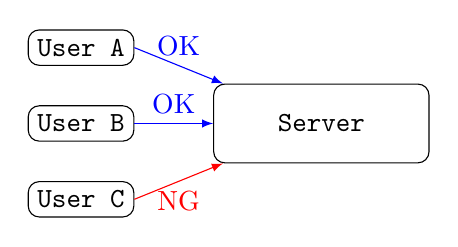
\begin{tikzpicture}
                            \tikzset{user/.style={draw,rounded corners,text centered}};
                            \node[user](userA){\tt User A};
                            \node[user,below=0.5cm of userA](userB){\tt User B};
                            \node[user,below=0.5cm of userB](userC){\tt User C};
                            \node[file,right=1cm of userB](server){\tt Server};
                            \foreach \u in{A,B}
                            \draw[-latex,blue](user\u.east)--(server)node[midway,above]{\textcolor{blue}{OK}};
                            \draw[-latex,red](userC.east)--(server)node[midway,below]{\textcolor{red}{NG}};
                        \end{tikzpicture}
                    \end{figure}
                \end{minipage}
            \end{block}
        \end{column}
        \begin{column}[t]{0.49\linewidth}
            \begin{block}{Authorization}
                \begin{minipage}[c][0.4\textheight][c]{\linewidth}
                    \begin{figure}[h]
                        \centering
                        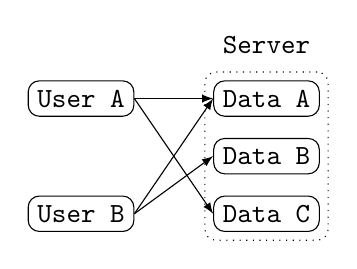
\begin{tikzpicture}
                            \node[user](userA){\tt User A};
                            \node[user,below=1cm of userA](userB){\tt User B};
                            \node[user,right=01cm of userA](dataA){\tt Data A};
                            \node[user,right=1cm of userB](dataC){\tt Data C};
                            \node[user] at ($(dataA)!0.5!(dataC)$)(dataB){\tt Data B};
                            \node[inner sep=3pt,fit={(dataA)(dataB)(dataC)},draw,dotted,rounded corners](warp_data){};
                            \node[above=0.1cm of warp_data]{\tt Server};
                            \foreach \u \v in {A/A,A/C,B/A,B/B}
                            \draw[-latex](user\u.east)--(data\v.west);
                        \end{tikzpicture}
                    \end{figure}
                \end{minipage}
            \end{block}
        \end{column}
    \end{columns}
\end{frame}
\subsection{OAuth}
\begin{frame}{\shownum OAuth}
    \begin{exampleblock}{OAuth}
        OAuth(Open Authorization) is system used to allow multiple web services to work together.
    \end{exampleblock}
    \begin{figure}[h]
        \centering
        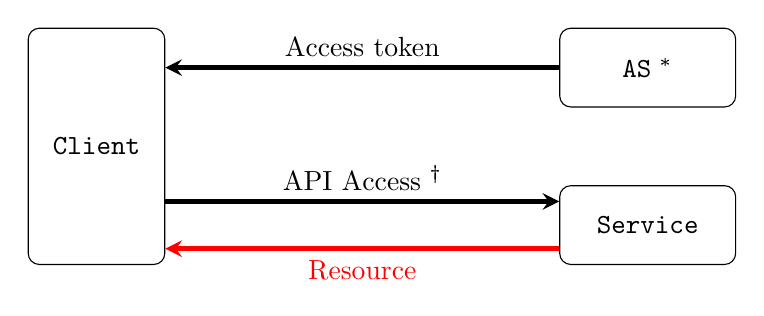
\begin{tikzpicture}
            \node[text centered,rounded corners,draw,minimum height=3cm,text width=1.5cm](client){\tt Client};
            \coordinate (S) at ($(client)+(7cm,0cm)$);
            \coordinate (S2) at (S |- client.west);
            \node[user,text width=2cm,minimum height=1cm] at ($(S2)+(0,1cm)$)(AS){\tt AS\ \footnotemark};
            \node[user,text width=2cm,minimum height=1cm] at ($(S2)+(0,-1cm)$)(service){\tt Service};
            \draw[ultra thick,-stealth](AS.west)--(client.east |- AS.west)node[midway,above]{Access token};
            \coordinate (S3) at ($(service.east)+(0,0.3cm)$);
            \coordinate (S4) at ($(service.east)+(0,-0.3cm)$);
            \draw[ultra thick,-stealth](client.east|-S3)--($(service.west)+(0,0.3cm)$)node[midway,above]{API Access \footnotemark};
            \draw[ultra thick,-stealth,red]($(service.west)+(0,-0.3cm)$)--(client.east|-S4)node[midway,below]{Resource};
        \end{tikzpicture}
    \end{figure}
    \footnotetext[1]{AS : Authorization Server}
    \footnotetext[2]{With an access token.}
\end{frame}
\begin{frame}{\shownum OAuth}
    \begin{block}{Access token issuance procedure}
        \begin{enumerate}
            \item The client sends an authorization request to authorization server via web browser, together with a client ID and a URI to redirect.
            \item The authorization server authenticates the user via a browser and outputs a "permission" acceptance screen.
            \item If the user allows it, the authorization server redirects the browser and sends authorization code to the client.
            \item The client server sends the authorization code and redirect URI to the authorization server.
            \item The authorization server authenticates the client, verifies the authorization code and redirect URI, and sends access token to the client.
        \end{enumerate}
    \end{block}
\end{frame}
\begin{frame}{\shownum OAuth}
    \begin{figure}
        \centering
        \caption*{OAuth 2.0 Authorization code ground}
        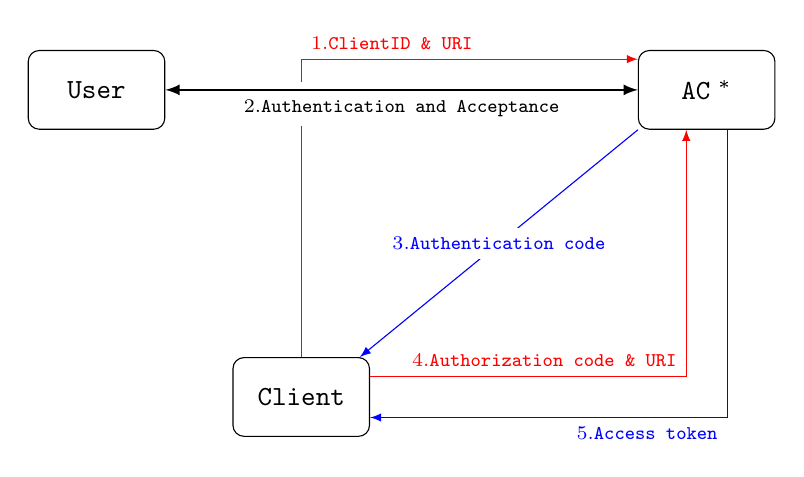
\begin{tikzpicture}[scale=1.3]
            \node[user,text width=1.5cm,minimum height=1cm](user){\tt User};
            \node[user,text width=1.5cm,minimum height=1cm]at($(user)+(2cm,-3cm)$)(client){\tt Client};
            \node[user,text width=1.5cm,minimum height=1cm,right=6cm of user](server){\tt AC\ \footnotemark[1]};
            \draw[-latex,red](client)|-($(server.west)+(0,0.3cm)$)node[midway,above right]{\scriptsize 1.{\tt ClientID \& URI}};
            \draw[line width=6pt,white,latex-latex](server.west)--(user.east);
            \draw[thick,latex-latex](server.west)--(user.east)node[midway,below,fill=white]{\scriptsize 2.{\tt Authentication and Acceptance}};
            \draw[-latex,blue](server.south west)--($(client.north east)+(-0.1cm,0)$)node[midway,fill=white]{\scriptsize 3.{\tt Authentication code}};
            \draw[-latex,red]($(client.east)+(0,0.2cm)$)-|($(server.south)+(-0.2cm,0cm)$)node[midway,above left]{\scriptsize 4.{\tt Authorization code \& URI}};
            \draw[-latex,blue]($(server.south)+(0.2cm,0cm)$)|-($(client.east)+(0,-0.2cm)$)node[midway,below left]{\scriptsize 5.{\tt Access token}};
        \end{tikzpicture}
    \end{figure}
    \footnotetext[1]{AC : Authentication Server}
\end{frame}
\end{document}